\documentclass[12pt]{article}
\usepackage[utf8]{inputenc}
\usepackage{geometry, amsmath, amsthm, latexsym, amssymb, graphicx, bm, pgfplots, float}
\usepackage{tikz}
\geometry{margin=1in, headsep=0.25in}

\parindent 0in
\parskip 12pt
\pgfplotsset{compat=1.17}

\begin{document}
\title{Exercício EAD0671}

%\thispagestyle{empty}

\begin{center}
    {\LARGE \bf Exercício 5} \\
    
    {\large Douglas Cardoso - 11766990}\\
EAD0671
\end{center}

\textbf{Ex. 5 \\
Cerca de 100 milhões de libras de jujubas são anualmente consumidas nos Estados Unidos e seu preço é de cerca de US\$ 0,50 por libra. Entretanto, como os produtores desse bem acham que seus rendimentos estão muito baixos, conseguiram convencer o governo de que uma política de sustentação de preços seria adequada. Em consequência, o governo passará a adquirir a quantidade necessária de jujubas para que o preço seja mantido no nível de US\$ 1 por libra. Mas a equipe econômica está preocupada com o impacto desse programa, pois não dispõe de nenhuma estimativa para a elasticidade da oferta ou da demanda das jujubas.}

\textbf{(a) Será que esse programa poderia custar ao governo mais de US\$ 50 milhões por ano? Sob quais condições? Esse programa poderia custar menos de US\$ 50 milhões por ano? Sob quais condições? Faça uma ilustração por meio de um diagrama.}

A resposta depende da \textit{elasticidade} das jujubas. Caso a elasticidade seja maior que \textit{0,5}, então o governo irá despender mais que US\$50 milhões por ano.  O contrário também é provável, isto é, o produto tendo elasticidade menor que \textit{0,5}, o aumento de preços não causará muita mudança na quantidade, e o governo terá menos "áreas" para compensar. O diagrama abaixo representa isso:

\begin{center}
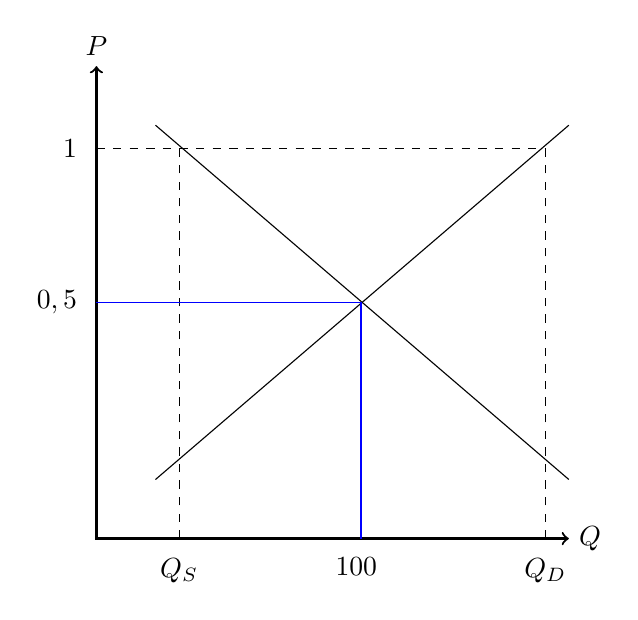
\begin{tikzpicture}[scale=3]
    \draw [<->, thick] (0,2) node (yaxis) [above] {$P$}
        |- (2,0) node (xaxis) [right] {$Q$};
        
    \draw (0.25,0.25) coordinate (a_1) -- (2, 1.75) coordinate (a_2);
    \draw (0.25,1.75) coordinate (b_1) -- (2, 0.25) coordinate (b_2);
    \draw[dashed] (0.35, 0) -- (0.35, 1.65);
    \node[label= below: {$Q_S$}] at (0.35, 0){};
    \draw[dashed] (1.9, 0) -- (1.9, 1.65);
    \node[label= below: {$Q_D$}] at (1.9, 0){};
    \draw[dashed] (0, 1.65) -- (1.9, 1.65);
    \node[label=left:{$1$}] at (0, 1.65){};
    \draw[draw=blue] (1.12,0) -- (1.12, 1);
    \draw[draw=blue] (0, 1) -- (1.12,1);
    \node[label=left:{$0,5$}] at (0, 1){};
    \node[label=below:{$100$}] at (1.1, 0){};
\end{tikzpicture}
\end{center}

No diagrama é possível observar que caso a diferença entre $Q_S$ e $Q_D$ seja maior que US\$ 50 milhões, então o governo pagará mais que US\$ 50 milhões.

\textbf{(b) Será que esse programa poderia custar aos consumidores (em termos de perda de excedente do consumidor) mais de US\$ 50 milhões por ano? Sob quais condições? Esse programa poderia custar aos consumidores menos de US\$ 50 milhões por ano? Sob quais condições? Novamente, faça uma ilustração por meio de um diagrama.}

O programa custaria exatamente US\$ 50 milhões ou menos aos consumidores, isto porque, se traçarmos uma curva de demanda perfeitamente inelástica cortando o ponto de equilíbrio do diagrama do item \textbf{(a)}, a perda do excedente do consumidor seria exatamente de US\$ 50 milhões ($1-0,5$), caso essa curva não seja assim, então a perda do excedente do consumidor será menor.

\begin{center}
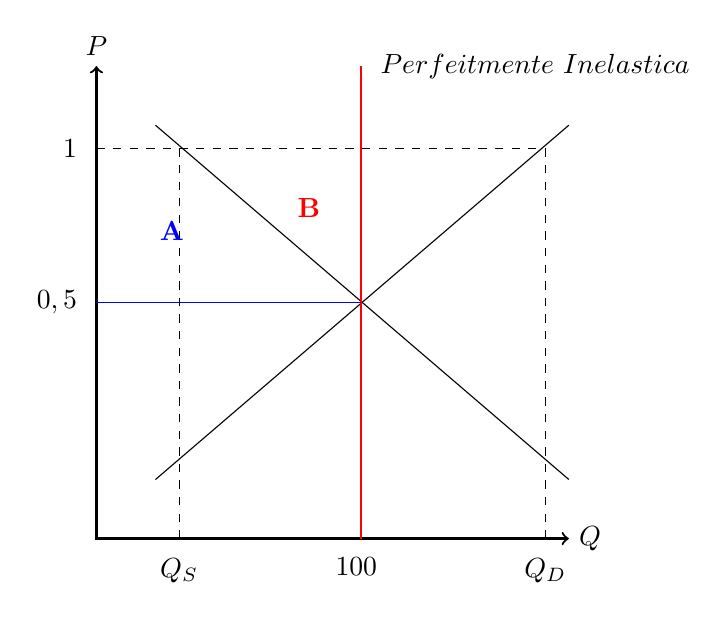
\begin{tikzpicture}[scale=3]
    \draw [<->, thick] (0,2) node (yaxis) [above] {$P$}
        |- (2,0) node (xaxis) [right] {$Q$};
        
    \draw (0.25,0.25) coordinate (a_1) -- (2, 1.75) coordinate (a_2);
    \draw (0.25,1.75) coordinate (b_1) -- (2, 0.25) coordinate (b_2);
    \draw[dashed] (0.35, 0) -- (0.35, 1.65);
    \node[label= below: {$Q_S$}] at (0.35, 0){};
    \draw[dashed] (1.9, 0) -- (1.9, 1.65);
    \node[label= below: {$Q_D$}] at (1.9, 0){};
    \draw[dashed] (0, 1.65) -- (1.9, 1.65);
    \node[label=left:{$1$}] at (0, 1.65){};
    \draw[draw=red] (1.12,0) -- (1.12, 2) node[red, label=right:{$Perfeitmente\ {Inelastica}$}] {};
    \node[label=left:{$0,5$}] at (0, 1){};
    \node[label=below:{$100$}] at (1.1, 0){};
    \draw[draw=blue] (0, 1) -- (1.12,1);
    \node[] at (0.32, 1.3){\textbf{\textcolor{blue}{A}}};
     \node[] at (0.9, 1.4){\textbf{\textcolor{red}{B}}};
\end{tikzpicture}
\end{center}
\end{document}
